% !TEX root = mythesis.tex

%==============================================================================
\chapter{Alignment}
\label{sec:align}
%==============================================================================
Measuring charged particles precisely and efficiently is a crucial part of any particle physics experiment. This need is intensified more for NA64 since we need a very accurate estimate for the beam momentum and energy to look for missing energy events for the \textit{invisible mode}. NA64 also requires an accurate track reconstruction for the \textit{visible mode} to look for $e^+ e^-$ tracks that might originate from a possible $A'$. While the experiment was being installed a big emphasis was given to measure the outer boundaries of the detectors using lasers. Nonetheless this precision is insufficient when extrapolated to get an estimate for the inner part of the detector. Since the detectors are expected to have a micrometer precision, track based alignment will provide a better estimate for the actual detector positions and will help improving the errors in the final physics analysis. This chapter describes the program \textbf{Millepede} implemented for the track based alignment for NA64 and also reports the different types of alignment performed for the current setup. The results of alignment program are also compared to the standalone alignment method described in \cite{nabeel:2018}.

\section{Previously used method}
\label{sec:prev_used}
The previously used method~\cite{nabeel:2018} which was used for alignment in NA64 is a simple residual fit and shift. A short description of the steps involved in this procedure is as follows:
\begin{enumerate}
    \item The raw data which contains the hit information along with the detectors table is fed to CORAL for track reconstruction. Kalman filter is used for track reconstruction.
    \item The output from the reconstruction is obtained in form of a mini data storage (mdst) format which is analysed using PHAST.
    \item Residuals are calculated and fitted with a standard Gauss function to extract the peak for the residuals. An example for a specific plane is shown in fig.(\ref{fig:res_GEM4x}). This procedure is performed for each plane of the detector.
    \item The fitted peaks are the shifts for the detectors and for a good alignment should be centered to zero. These shifts are applied to the detectors table. For the next iteration the new updated detectors table is used as an input to CORAL.
    \item The number of iterations are selected by looking at the change in the reduced chi-square. This procedure is not automated at this point.
\end{enumerate}
Such a procedure has many limitations and can even lead to situations where there are simultaneous shifts in opposite directions. This procedure can only align for the X and Y planes of the detector and is not currently structured to include rotation of the planes of the detector. These problems are described in detail by V.Blobel in \cite{Blobel:2006yh}.

\begin{figure}[t!]
\centering
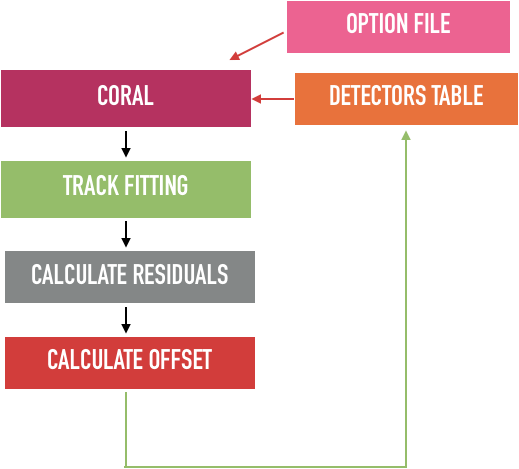
\includegraphics[width=0.65\textwidth]{thesis_figures/Previous_method.png}
\caption{Pictorial representation of the previously used method}
\label{fig:previously_used_flowchart}
\end{figure}

\begin{figure}[t!]
\centering
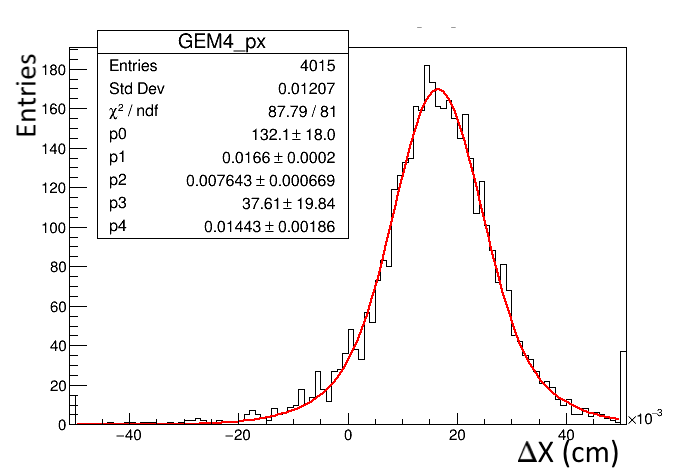
\includegraphics[width=0.65\textwidth]{thesis_figures/alignment/Residual_GEM4X.png}
\caption{Fitting of the residual for the X plane of GEM4}
\label{fig:res_GEM4x}
\end{figure}
%\FloatBarrier
\section{Millepede}
Millepede is an iterative alignment program that uses the linear least square method to fit and minimize all the relevant alignment parameters. The method and the initial implementation was developed by V. Blobel from the University of Hamburg and is maintained by  Deutsches Elektronen-Synchrotron (DESY) \cite{Millepede}. It is a smarter implementation of the previously used method that decreases the computation time while giving comparable results. The alignment parameters that Millepede tries to minimize can be seperated into two categories: \textit{global} and \textit{local}. Global parameters consist of sets of values that affect all data such as expected shifts for the detectors. On the other hand local parameters are values that are concerned with a single track such as slope, curvature etc. The previously used method ignores the global parameters and only aligns using individual tracks from measured events. If one of the detectors has a lot of noise for some reason the iterative residual based alignment may fail. This and many other reasons such as an inability to tangle correlated parameters while aligning makes the previously used method inferior compared to Millepede.

Following is the mathematical description of the Millepede algorithm which is closely adapted from \cite{Blobel:2002ax,Blusk:2007zza}.
Let the local parameters be denoted by $l_j$ where j is the  running index dependent on the complexity with which the track is described. For a general measurement the set of measurements at a detector plane k is given by
\begin{equation}
  y_k = l_1 \cdot \delta_{1k} + l_2 \cdot \delta_{2k} + ...l_n \cdot \delta_{nk} = \sum_{j=1}^n l_j \cdot \delta_{jk}
\end{equation}
where $\delta_j$ are some known constant factors. For example if the track measured at a detector, at position k, is a straight line track then: $y_k = l_1 \cdot 1 + l_2 \cdot S_k  $, where $l_1$ is the intercept and $l_2$ is the slope of the measured track. Here we assumed that the measurements are only dependent on local parameters. Similarly if we include global parameters $g_j$ then
\begin{equation}
  y = l_1 \cdot \delta_{1} + l_2 \cdot \delta_{2} + ...l_n \cdot \delta_{n} + g_1 \cdot h_{1} + g_2 \cdot h_{2} + ...g_n \cdot h_{u} = \sum_{j=1}^n l_j \cdot \delta_{j} + \sum_{i=1}^u g_i \cdot h_i .
\end{equation}
Linearising the above equation for a single point measured at location $x_i$ and track $k$ yields:
\begin{equation}
  y = f(x_i;\textbf{g},\textbf{l}) + \Bigg(  \frac{\partial f(x)}{\partial \textbf{g}_i} = d_i^{global} \Bigg)^T  \Delta\textbf{g} + \Bigg( \frac{\partial f(x)}{\partial \textbf{l}_i} = d_i^{local} \Bigg)^T  \Delta\textbf{l}_k
\end{equation}
with $f(x_i;\textbf{g},\textbf{l})$ being the mathematical model predicting the track and $\Delta\textbf{g}$ and $\Delta\textbf{l}$ are the corrections applied to global and local parameters after one iteration of a track fit.

The least square method requires us to solve the following matrix equation:
\begin{equation}
\begin{bmatrix}
    \sum_k C_k^{global} & \dots & H_k^{global-local} & \dots \\
    \vdots & \ddots & 0 & 0 \\
    (H_k^{global-local})^T & 0 & C_k^{local} & 0 \\
    \vdots & 0 & 0 & \ddots
\end{bmatrix}
\times
\begin{bmatrix}
    \Delta \textbf{g} \\
    \vdots  \\
    \Delta \textbf{l}_k \\
    \vdots
\end{bmatrix}
=
\begin{bmatrix}
    \sum_k b_k^{global}  \\
    \vdots  \\
    b_k^{local} \\
    \vdots
\end{bmatrix}
\end{equation}
here C is a symmetric matrix formulated as $C = \sum_{k=1}^m w_k d_k d_k^T $ with $w_k = 1/\sigma_k^2$ being the weight assigned to each measurement and $m$ being the total number of global parameters being fitted and $d_k$ being the derivative of the model with respect to the global parameter. A similar formulation is made for local parameters. $H_k$ is a matrix formulated in a similar way as to C and is defined as $H= \sum_k w_k d_k^{global} (d_k^{local})^T$. $b$ is the correction vector defined as $b = \sum_k w_k r_k d_k$ with $r_k$ being the residual as defined in sec.(\ref{sec:Linear_Regression}).

The Millepede algorithm implements a simultaneous fit for all tracks, including both local and global parameters. Since we only care about corrections to the global parameters the computation is sped up by focusing on $\Delta\textbf{g}$ calculation for each iterative step and solving the equation $\Delta\textbf{g} = (C^{global})^{-1} b^{global}$.

The step by step process of the Millepede minimization can be explained as follows:
\begin{enumerate}
    \item Fit the track using a fitter such as Kalman and extract the best values for local parameters.
    \item Collect derivatives $d_k$ for all local and global parameters that need to be minimized.
    \item Update the matrices $C^{global}$ and $b^{global}$ for each track by simple addition. An extra step is needed to update matrix $C:= C - HVH^T$ which indirectly includes the changes applied to the local parameters while updating the global parameters.
    \item Repeat the above steps for all the available tracks.
\end{enumerate}

After all the tracks have been computed and the relevant global matrices have been calculated the final equation $\Delta\textbf{g} = (C^{global})^{-1} b^{global}$ is solved. The inversion while calculating this equation is made even faster by partitioning the matrix into symmetric sub-matrices which is one of the special features of Millepede and is described in detail in \cite{Blobel:2002ax}.

The whole process of looping over all tracks and then computing the correction to the global parameters counts as one iteration of the Millepede algorithm. The selection for the number of iterations depends on the number of global parameters being used and the correlation between them if any.


\section{CORAL Implementation}
The Millepede program is included as a separate library "millepede.f"  in CORAL. The algorithm is written in FORTRAN and H.Pereira \cite{PereiraDaCosta:1204557} introduced an interface for the algorithm into CORAL. The options available for global parameters that can be minimized are positional(U) alignment, angular(T) alignment, pitch(P) alignment, alignment for the z position of the detector along the beam and many more which are not relevant for our tracking detectors.

\begin{figure}[t!]
\centering
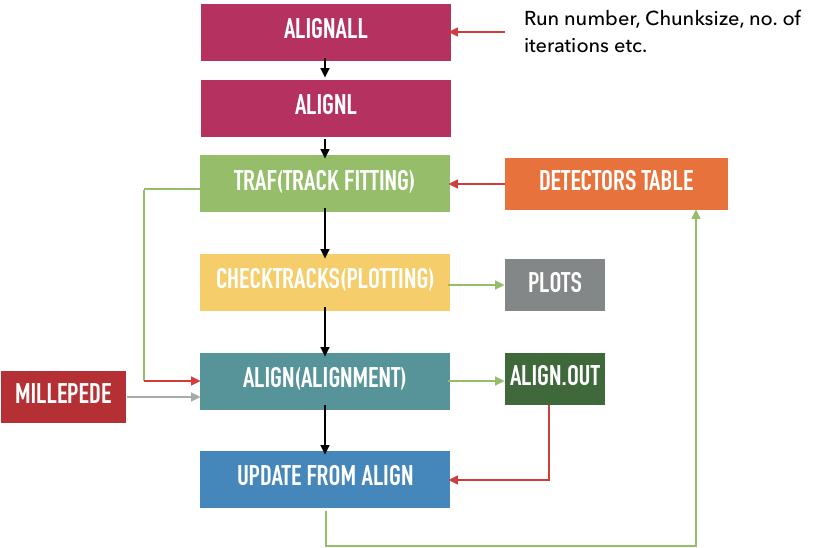
\includegraphics[width=\textwidth]{thesis_figures/Millepede_implementation.png}
\caption{ CORAL implementation of Millepede. The black lines signify the order of the steps while the green and red lines depict output and input respectively.}
\label{fig:millepede_implementation}
\end{figure}


The alignment method used in CORAL works on the standard Millepede condition which minimizes the sum of $\chi^2_{red}$ with respect to the local and global parameters. The method in CORAL is controlled using separate option files similar to the ones used in track fitting. The data flow for the whole alignment process is described in fig.(\ref{fig:millepede_implementation}).
\begin{description}
    \item $\Rightarrow$ "Alignall" and "Alignl" are bash scripts which are used in standard COMPASS alignment for staging the required data files for which the alignment needs to be performed. They also stage external files that CORAL needs such as the Dico file (faster bridging) for track fitting. The bash scripts are also involved in data management and in cleaning up of intermediate files produced during the alignment procedure. The bash scripts control the data flow and invoke different option files. the process begins by invoking the track fitting in CORAL which starts the alignment procedure. These scripts were adapted to work with NA64 and new options were introduced for the experiment.

    \item $\Rightarrow$ Track fitting uses the standard option file used for track reconstruction in NA64 with a few extra options. The most important option that is required to fill the root trees on which alignment works is "main do alignment". Other options such as whether to use the magnets and tracks having a non-zero momentum for alignment can also be set depending on the requirements. Both of these were used for the results mentioned in this thesis.

    \item $\Rightarrow$ Next the "checktracks" option is called. This option is used for plotting and checking the effect of each alignment step. It helps to achieve an immediate quality check and can be useful to spot errors in track reconstruction. It also gives basic information such as the alignment performance per iteration. For the first iteration step it gives the results of track reconstruction done on the setup where no software alignment was performed.

    \item $\Rightarrow$ Further, the "align" option is summoned. The "align" option is fed with the track reconstruction output from CORAL along with the detector positions. Moreover, the kind of global parameters that need to be minimized are specified at this stage. Other options such as aligning specific detectors, track selection cuts and inputting specific detector resolutions are also available. The Millepede minimization is invoked at this point. The "align" option gives an output with the required correction for each detector, for the particular global parameter that was aligned.

    \item $\Rightarrow$ Next the output from the "align" option is fed to "updateFromAlign". This tool applies the correction to the detectors table to create a new "detectors.dat" which is used for track fitting in the next iteration if multiple alignment iterations are performed.
\end{description}


\section{Results}
The alignment procedure was performed for the data collected during the 2017 invisible mode run for NA64. During this period, data taking and calibration were performed using a 100 GeV $e^-$ beam. The results of the alignment were tested by performing track fitting on the last obtained detectors table after all Millepede iterations were completed. The tracks used to obtain the quantifiable values for judging the results were chosen such that one hit from \textbf{each} detector plane contributed to the fitted track. In 2017 there were four Micromegas (MM1-MM4) upstream of the magnets and two Micromegas (MM5-MM6) and four GEMs (GEM1-GEM4) downstream of the magnets. The total number of detector planes available during the NA64 operational period were 19 since the Y plane of GEM3 was not operational. Since both the track fitting and alignment processes use detector resolution during minimization it is important to mention that for these results the resolution for GEMs was fixed at 50$\mu m$ and for Micromegas it was fixed to be 100$\mu m$. A random physics run with number 3211 was chosen to observe the results of the procedure. The results from this run were also compared to the ones obtained by the previously used procedure in \cite{nabeel:2018}. 500000 events per run were analyzed and CASTOR file system was used to access the data to study the process for a future run-by-run alignment application on the CERN computer cluster (lxplus). Different global parameters were minimized to study their individualized effects. The final conclusion about the quality of the alignment was drawn upon by looking at the reduced chi-square~ $\chi^2_{red}$ distribution and the distribution of residuals.

\subsection[Positional Alignment]%
{Positional Alignment} %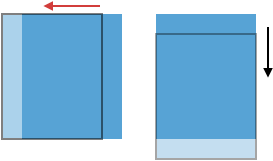
\includegraphics[width=20mm]{thesis_figures/positional.png}}

\begin{figure}[t!]
\centering
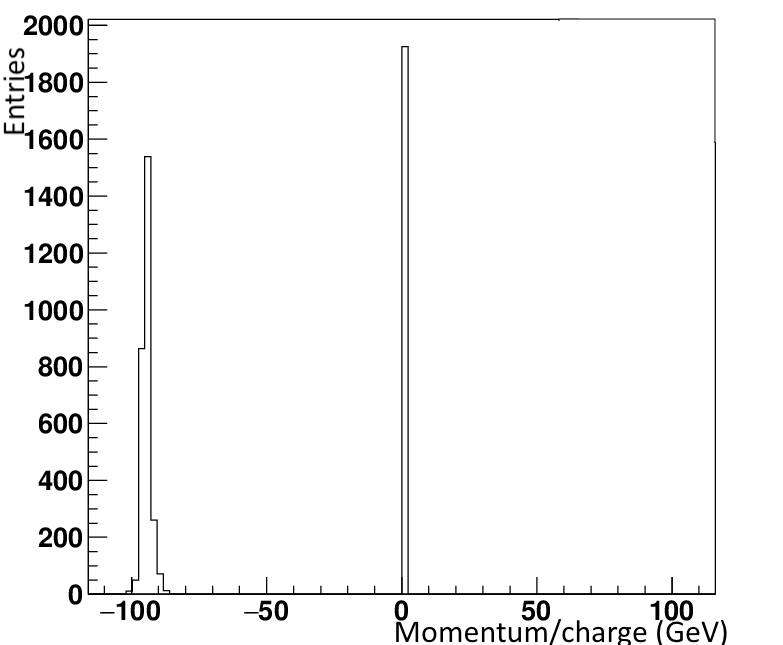
\includegraphics[width=0.65\textwidth]{thesis_figures/alignment/cop.png}
\caption{Charge over momentum distribution of all fitted tracks during alignment}
\label{fig:cop}
\end{figure}

The first global parameter which was aligned using the Millepede algorithm were the X and Y positions of the tracking detectors. In CORAL each readout plane of the detector is available to be aligned individually.
Positional(U) alignment refers to the alignment done to achieve an optimal (x,y) position for each detector plane. During the U alignment all detector planes were left free for movement in the (x,y) positions. However, other positional variables such as the angle with respect to the geometric reference system, z position and the pitch of the detectors were fixed. The tracks used for alignment were chosen to have $\chi^2_{red} < 100$ and a $-110 \text{GeV} <\text{p/charge}< -90 \text{GeV}$. The momentum over charge cut fig.(\ref{fig:cop}) made sure that only tracks that were bridged through the magnets were used for alignment. The results from the alignment are shown in figures (\ref{fig:GEM_residuals}), (\ref{fig:MX_residuals_1}) and (\ref{fig:MX_residuals_2}).

Ideally the residual distribution for a perfectly aligned detector should be centered around (0,0) which signifies that the measured hit position is accurately fitted during the track fitting procedure. As it can be seen from the figures, initially the residual distribution of almost all the detectors is displaced. Even though the observed displacement is small O(0.02cm), such a shift can hamper the positional resolution of the detectors which is expected to be of the O(~$\mu$m). This provides us with a visual proof that a software alignment is very much necessary. The final residual distribution after the Millepede alignment is much more uniform and is mostly centered around (0,0). The effect of the alignment is also measured by calculating the $\chi_{red}^2$ of all the selected tracks before and after alignment. We see in fig.(\ref{fig:red_chi2_1}) that the distribution shifts to a lower value which signifies that the alignment resulted in tracks with a lower $\chi_{red}^2$ i.e a better fit.

 The Millepede implementation was also compared to the previously used method (sec.(~\ref{sec:prev_used})). The $\chi_{red}^2$ comparison is shown in fig.(\ref{fig:red_chi2_2}). We again observe a lower $\chi_{red}^2$ distribution for the tracks in comparison to the one from the previously used method, though in this case the difference is not as drastic as the one seen before. This figure gives us a quantitative indication that the Millepede alignment method is in-fact better than the one which was previously used, which was expected. Although, the difference between the methods is not very large which shows that the previously used alignment method gives a reasonable detector alignment.
The individual residual distributions of the detectors for the previously used method are presented in appendix (\ref{sec:app_1}).

Looking closely at the residual distribution for the GEM detectors in fig.(\ref{fig:GEM_residuals}) one also observes a strange correlation between the residuals of the two planes. This behaviour is not expected since residuals in individual planes of the same detector should ideally be independent of each other (perpendicular strips). Such a distribution might be observed if there is an inherent angle between the two strip layers which even though highly unlikely cannot be completely ignored. This explanation is checked using angular alignment in the next section. Another reason for this behaviour might be due to our Micromega detectors. As mentioned before these detectors are set up such that they are rotated by a $45^{\circ}$ angle with respect to the global reference system which is also the reference system of the GEMs. Since the observed correlation also has an approximate angle similar to that of this rotation, the bad resolution of the Micromegas particularly in one plane as explained earlier might be the reason of these observations. This reasoning was checked by refitting the tracks and recalculating the residuals for the GEMs for the case where MM5 and MM6, the two downstream Micromegas were switched off and not used during the track reconstruction. The results of this check can be seen in fig.(\ref{fig:MX_off}). From the figure it is clear that the correlation in GEMs was due to the downstream Micromegas. Once they are switched off we are still left with a fairly large spread for the X residual, this might be due to the spread in the momentum when the beam passes through the magnet since X is the bending plane for our magnetic field.
The increased events observed in the histograms on the right are due to the total number of events analysed in the run which was doubled while performing the initial track fitting.

%\newpage
\begin{figure}[h!]
\centering
 \begin{subfigure}[l]{.45\textwidth}
   \centering
   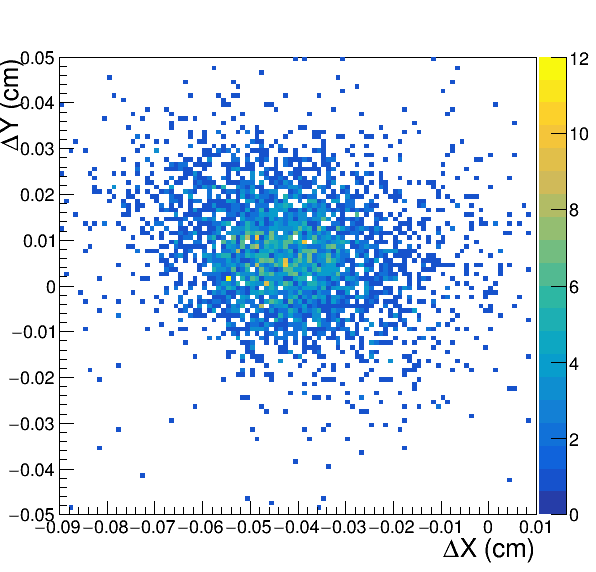
\includegraphics[width=\linewidth]{thesis_figures/alignment/Run_3211_before/square/GEM1.png}

   \caption{GEM1 before alignment}
   \label{fig:GEM1_before}
 \end{subfigure}
 %\hfill
 \begin{subfigure}[r]{.45\textwidth}
   \centering
   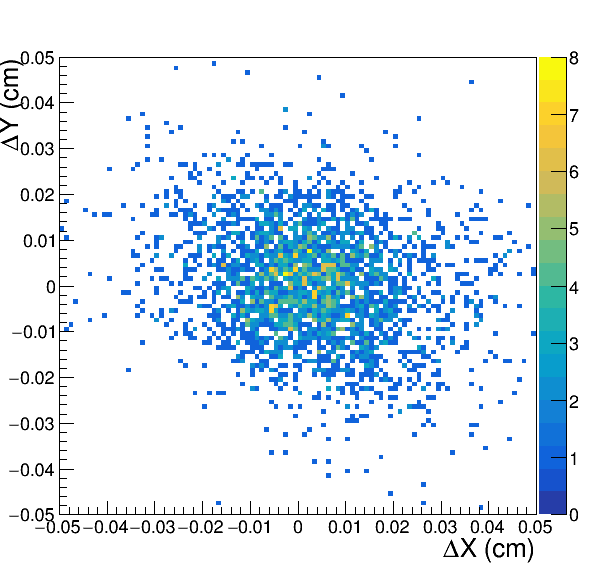
\includegraphics[width=\linewidth]{thesis_figures/alignment/Run_3211_after_millepede/square/GEM1.png}
   \caption{GEM1 after Millepede}
   \label{fig:GEM1_after}
 \end{subfigure}
 \hfill
 \begin{subfigure}[l]{.45\textwidth}
   \centering
   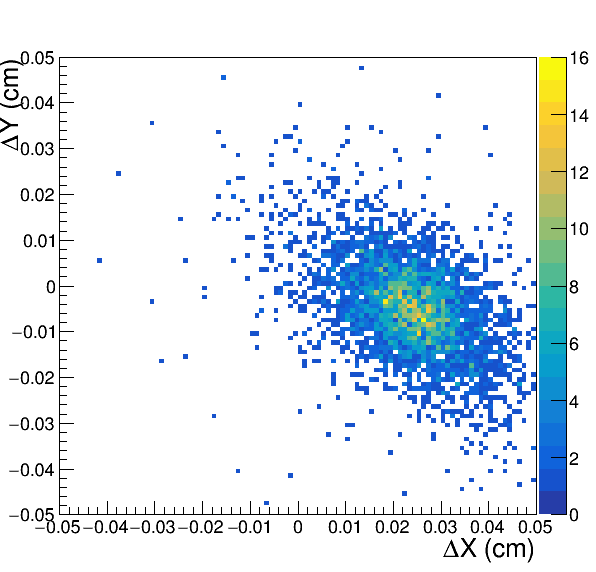
\includegraphics[width=\linewidth]{thesis_figures/alignment/Run_3211_before/square/GEM2.png}
   \caption{GEM2 before alignment}
   \label{fig:GEM2_before}
 \end{subfigure}
 %\hfill
 \begin{subfigure}[r]{.45\textwidth}
   \centering
   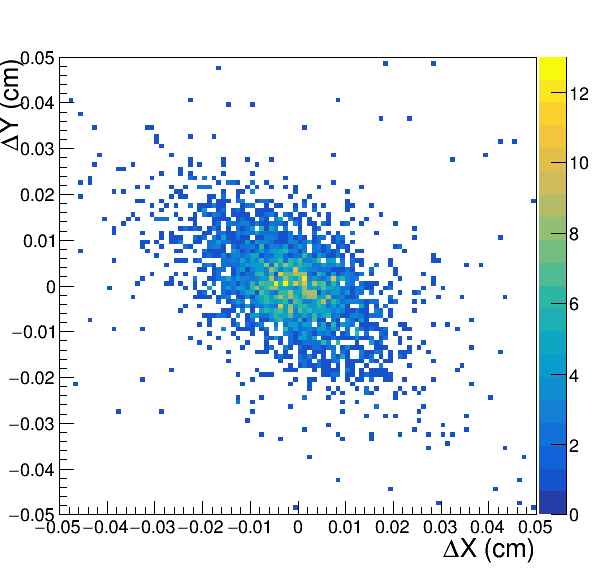
\includegraphics[width=\linewidth]{thesis_figures/alignment/Run_3211_after_millepede/square/GEM2.png}
   \caption{GEM2 after Millepede}
   \label{fig:GEM2_after}
 \end{subfigure}
 \begin{subfigure}[l]{.45\textwidth}
   \centering
   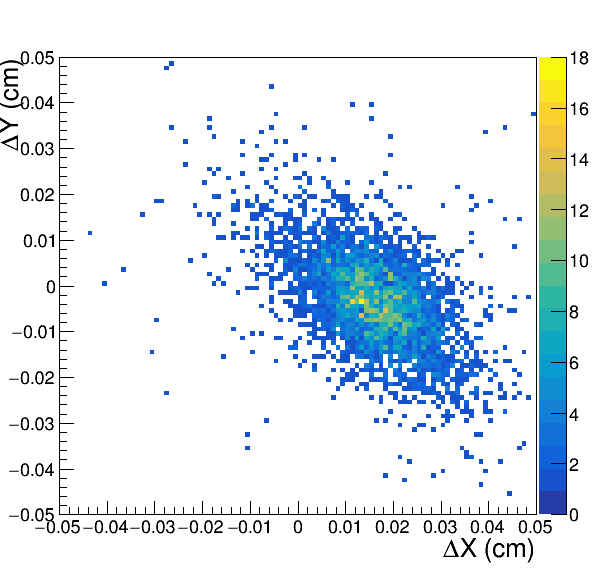
\includegraphics[width=\linewidth]{thesis_figures/alignment/Run_3211_before/square/GEM4.png}

   \caption{GEM4 before alignment}
   \label{fig:GEM4_before}
 \end{subfigure}
 %\hfill
 \begin{subfigure}[r]{.45\textwidth}
   \centering
   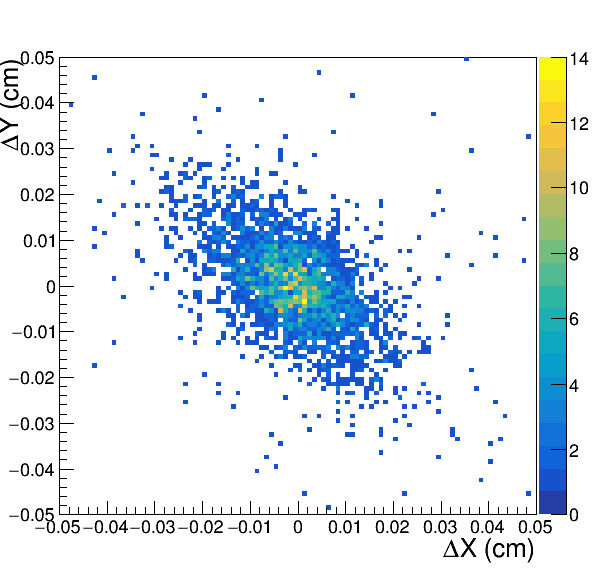
\includegraphics[width=\linewidth]{thesis_figures/alignment/Run_3211_after_millepede/square/GEM4.png}
   \caption{GEM4 after Millepede}
   \label{fig:GEM4_after}
 \end{subfigure}
 \caption{Residual of GEM detectors}
 \label{fig:GEM_residuals}
\end{figure}

%%%%MICROMEGAS start here

\begin{figure}[h!]
\centering
 \begin{subfigure}[l]{.45\textwidth}
   \centering
   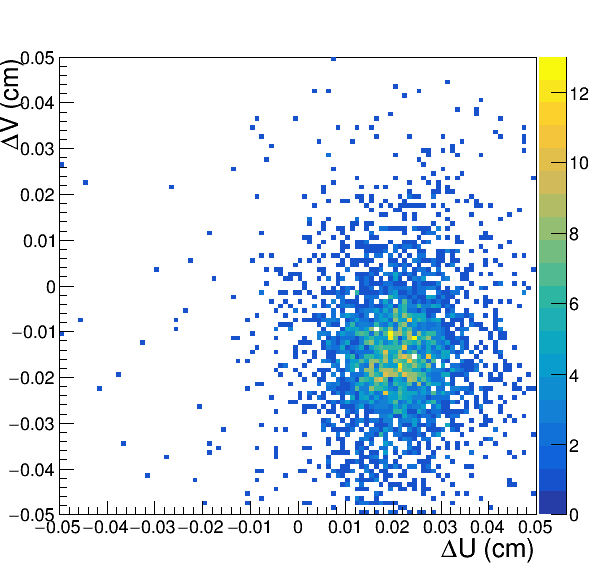
\includegraphics[width=\linewidth]{thesis_figures/alignment/Run_3211_before/square/MX1.png}

   \caption{MM1 before alignment}
   \label{fig:MX1_before}
 \end{subfigure}
 %\hfill
 \begin{subfigure}[r]{.45\textwidth}
   \centering
   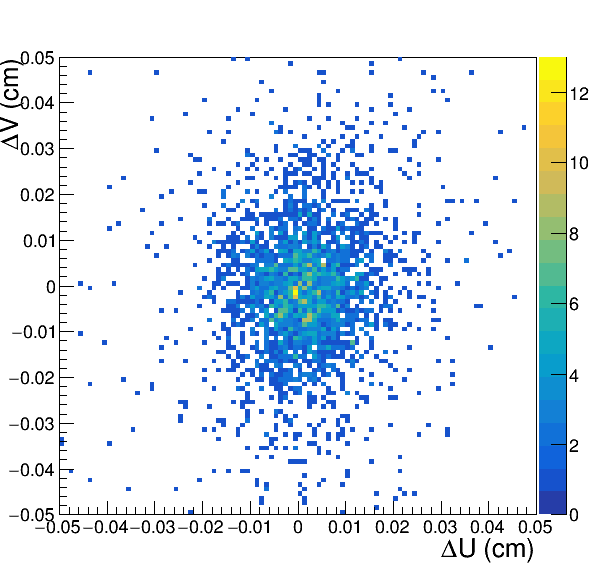
\includegraphics[width=\linewidth]{thesis_figures/alignment/Run_3211_after_millepede/square/MX1.png}
   \caption{MM1 after Millepede}
   \label{fig:MX1_after}
 \end{subfigure}
 \hfill
 \begin{subfigure}[l]{.45\textwidth}
   \centering
   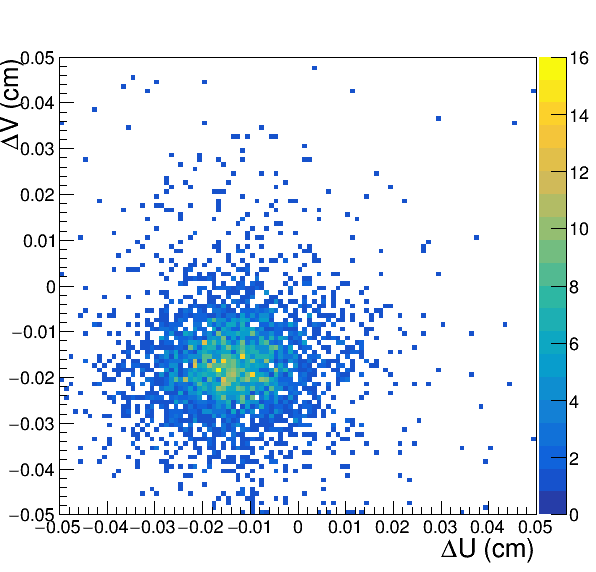
\includegraphics[width=\linewidth]{thesis_figures/alignment/Run_3211_before/square/MX2.png}
   \caption{MM2 before alignment}
   \label{fig:MX2_before}
 \end{subfigure}
 %\hfill
 \begin{subfigure}[r]{.45\textwidth}
   \centering
   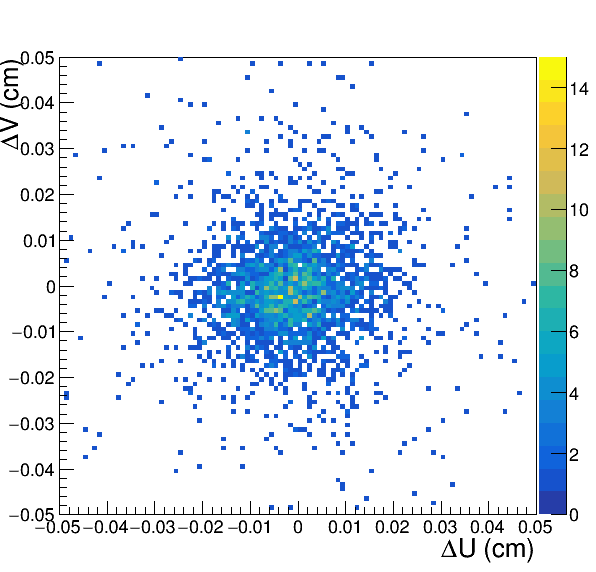
\includegraphics[width=\linewidth]{thesis_figures/alignment/Run_3211_after_millepede/square/MX2.png}
   \caption{MM2 after Millepede}
   \label{fig:MX2_after}
 \end{subfigure}
 \begin{subfigure}[l]{.45\textwidth}
   \centering
   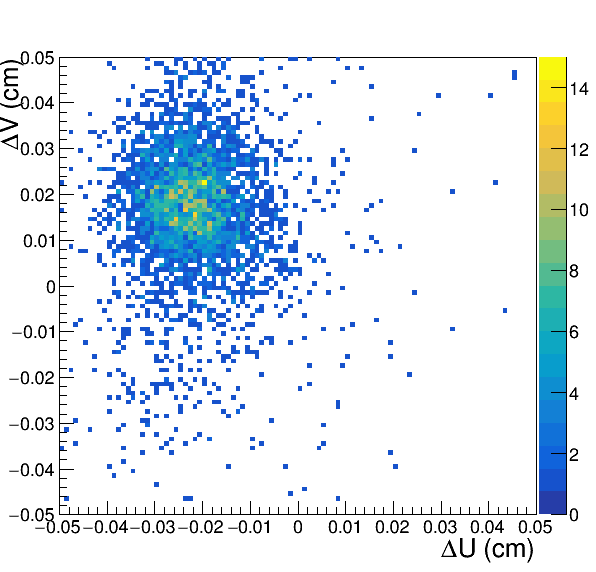
\includegraphics[width=\linewidth]{thesis_figures/alignment/Run_3211_before/square/MX3.png}

   \caption{MM3 before alignment}
   \label{fig:MM3_before}
 \end{subfigure}
 %\hfill
 \begin{subfigure}[r]{.45\textwidth}
   \centering
   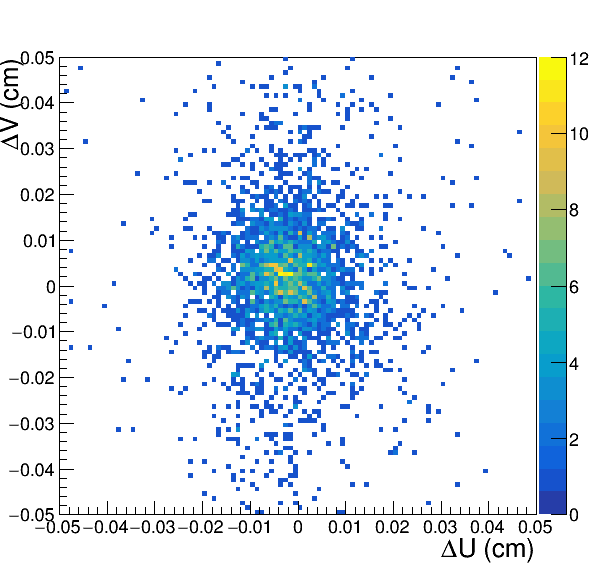
\includegraphics[width=\linewidth]{thesis_figures/alignment/Run_3211_after_millepede/square/MX3.png}
   \caption{MM3 after Millepede}
   \label{fig:MX3_after}
 \end{subfigure}
 \caption{Residual of Micromega detectors}
  \label{fig:MX_residuals_1}
\end{figure}


\begin{figure}[h!]
\centering
 \begin{subfigure}[l]{.45\textwidth}
   \centering
   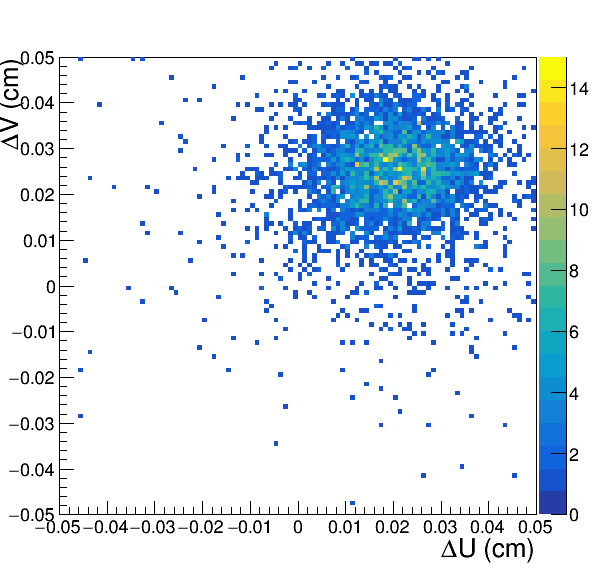
\includegraphics[width=\linewidth]{thesis_figures/alignment/Run_3211_before/square/MX4.png}

   \caption{MM4 before alignment}
   \label{fig:MX4_before}
 \end{subfigure}
 %\hfill
 \begin{subfigure}[r]{.45\textwidth}
   \centering
   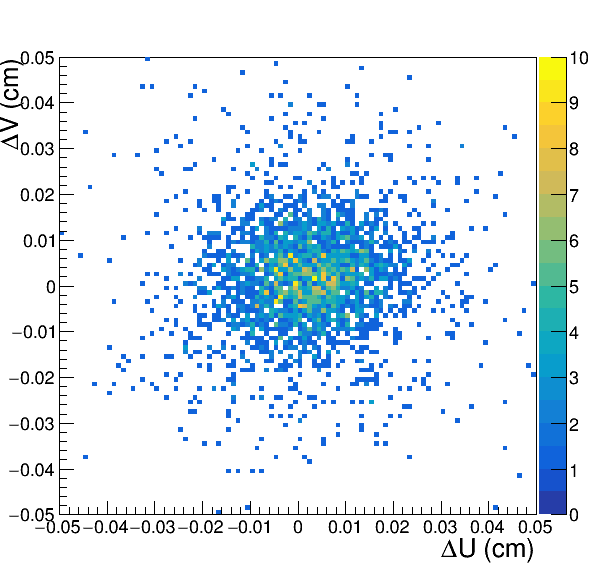
\includegraphics[width=\linewidth]{thesis_figures/alignment/Run_3211_after_millepede/square/MX4.png}
   \caption{MM4 after Millepede}
   \label{fig:MX4_after}
 \end{subfigure}
 \hfill
 \begin{subfigure}[l]{.45\textwidth}
   \centering
   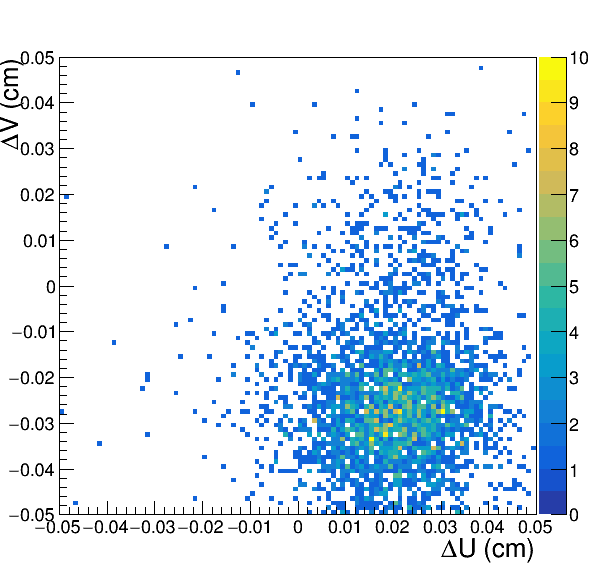
\includegraphics[width=\linewidth]{thesis_figures/alignment/Run_3211_before/square/MX5.png}
   \caption{MM5 before alignment}
   \label{fig:MX5_before}
 \end{subfigure}
 %\hfill
 \begin{subfigure}[r]{.45\textwidth}
   \centering
   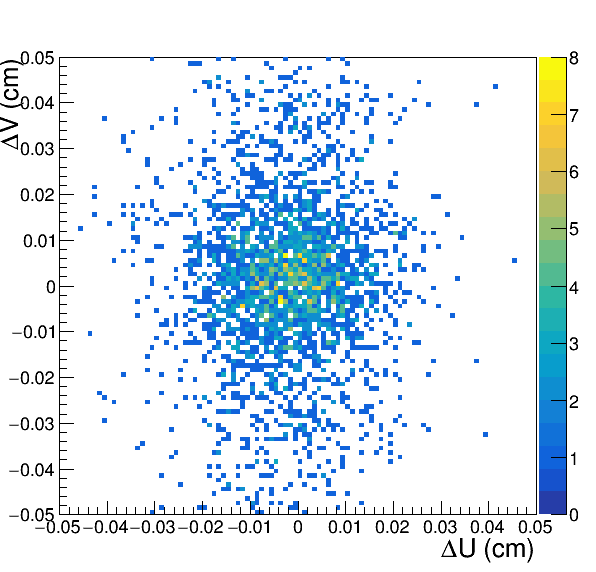
\includegraphics[width=\linewidth]{thesis_figures/alignment/Run_3211_after_millepede/square/MX5.png}
   \caption{MM5 after Millepede}
   \label{fig:MX5_after}
 \end{subfigure}
 \begin{subfigure}[l]{.45\textwidth}
   \centering
   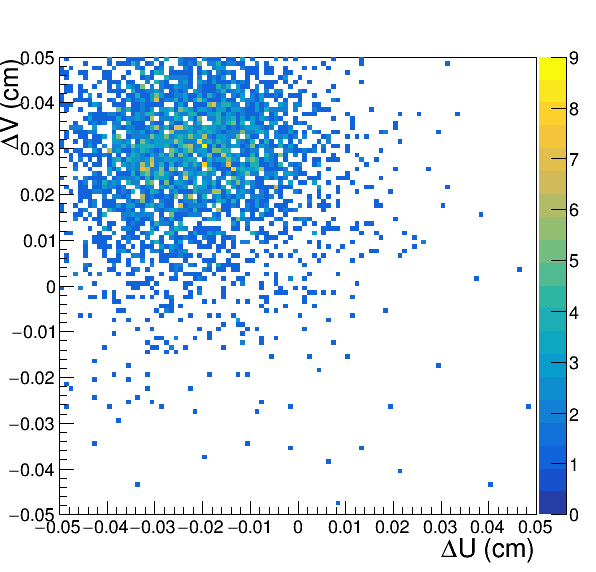
\includegraphics[width=\linewidth]{thesis_figures/alignment/Run_3211_before/square/MX7.png}

   \caption{MM6 before alignment}
   \label{fig:MX6_before}
 \end{subfigure}
 %\hfill
 \begin{subfigure}[r]{.45\textwidth}
   \centering
   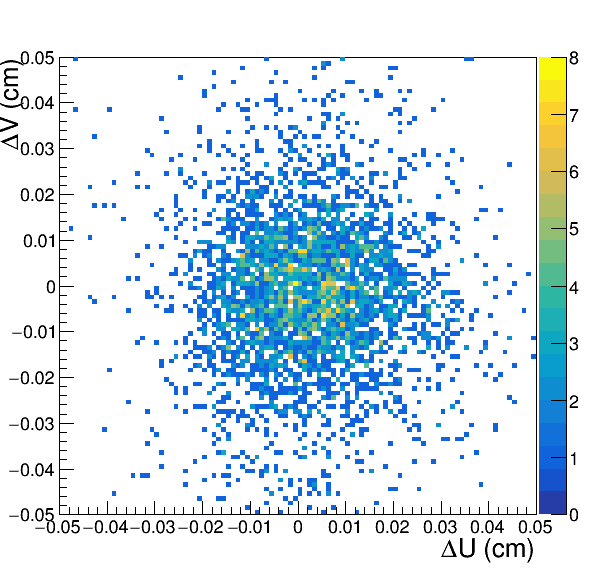
\includegraphics[width=\linewidth]{thesis_figures/alignment/Run_3211_after_millepede/square/MX7.png}
   \caption{MM6 after Millepede}
   \label{fig:MX6_after}
 \end{subfigure}
 \caption{Residual of Micromega detectors}
 \label{fig:MX_residuals_2}
\end{figure}

\begin{figure}[h!]
\centering
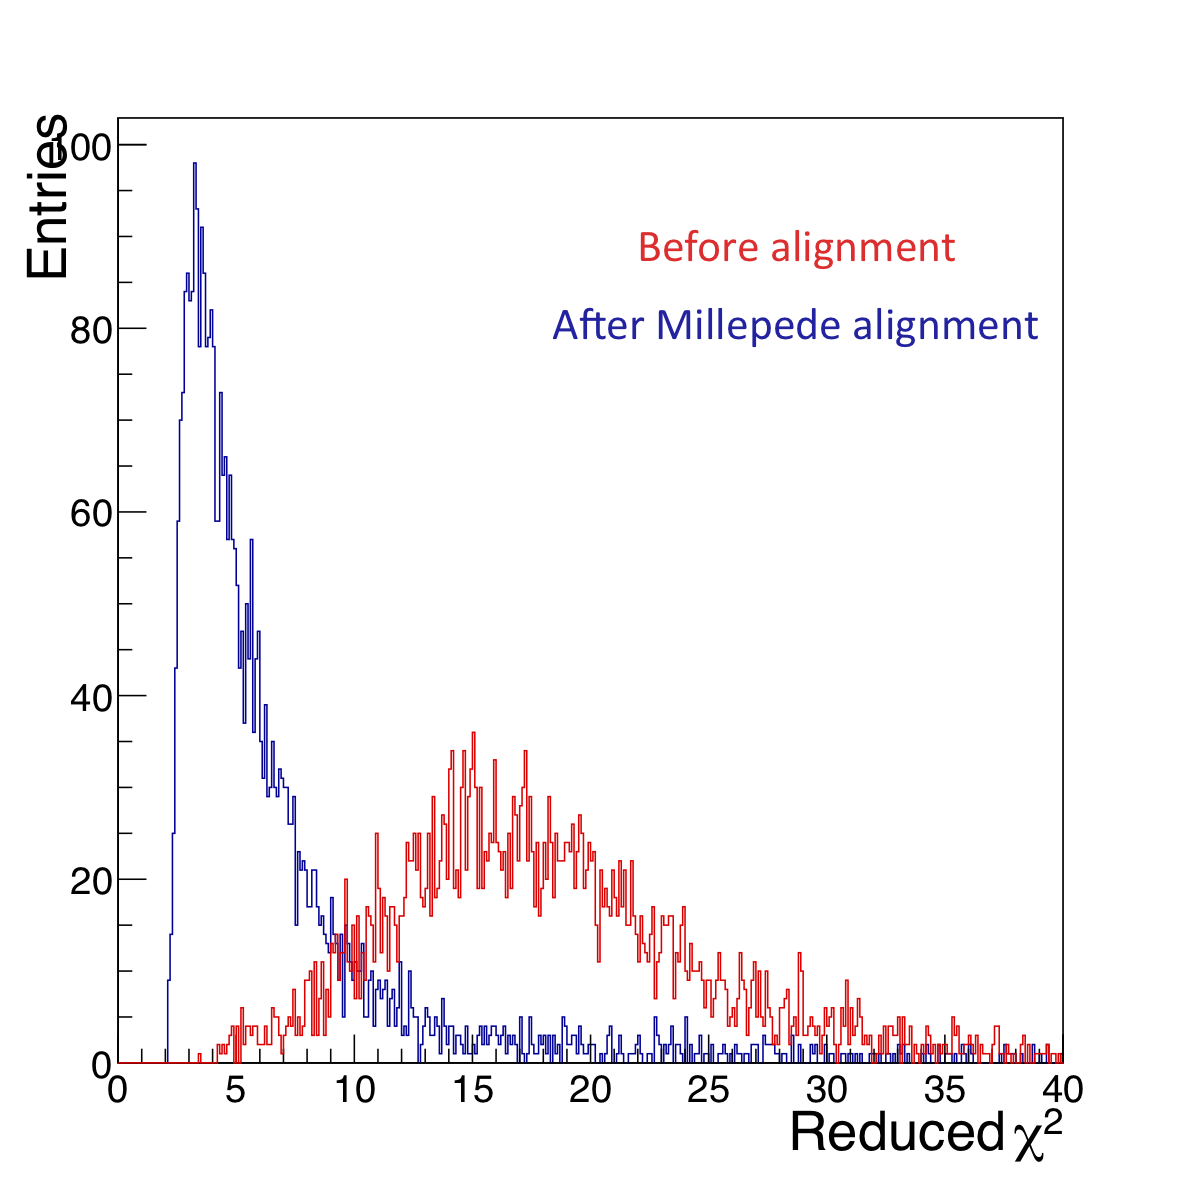
\includegraphics[width=0.6\textwidth]{thesis_figures/alignment/red_chi2_bvs_after_square.png}
\caption{$\chi_{red}^2$ comparison before and after Millepede alignment implementation}
\label{fig:red_chi2_1}
\end{figure}

\begin{figure}[h!]
\centering
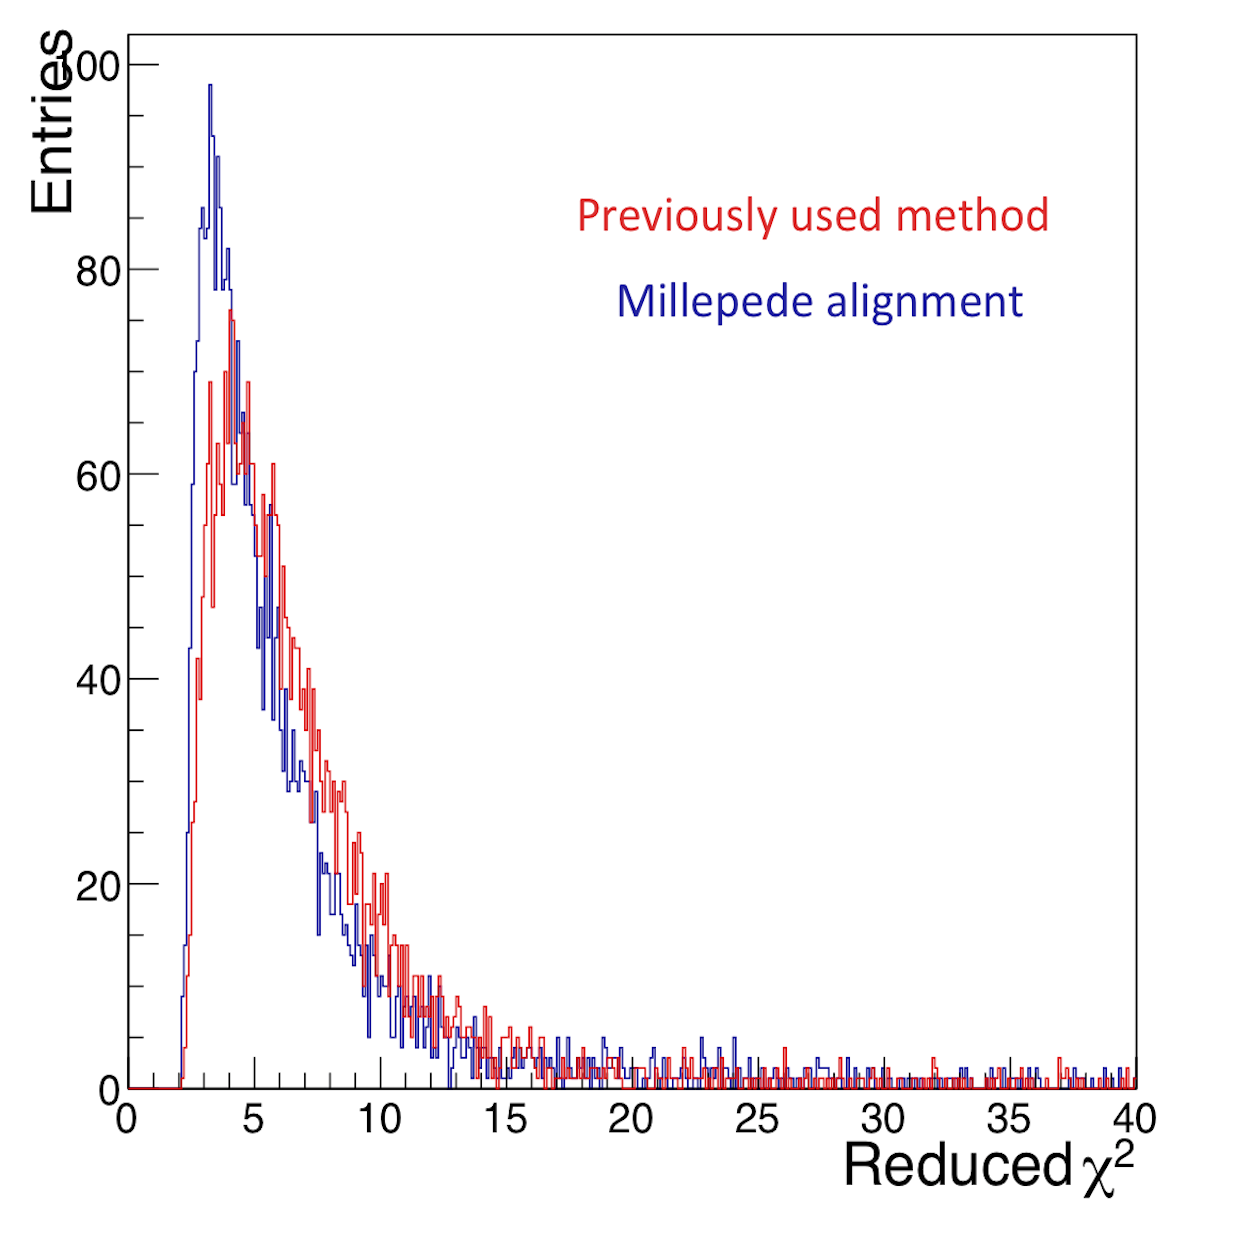
\includegraphics[width=0.6\textwidth]{thesis_figures/alignment/red_chi2_navsm_final.png}
\caption{$\chi_{red}^2$ comparison of previously used method with Millepede alignment implementation}
\label{fig:red_chi2_2}
\end{figure}

%%Micromegas off and not off
\begin{figure}[h!]
\centering
\begin{subfigure}[l]{.45\textwidth}
  \centering
  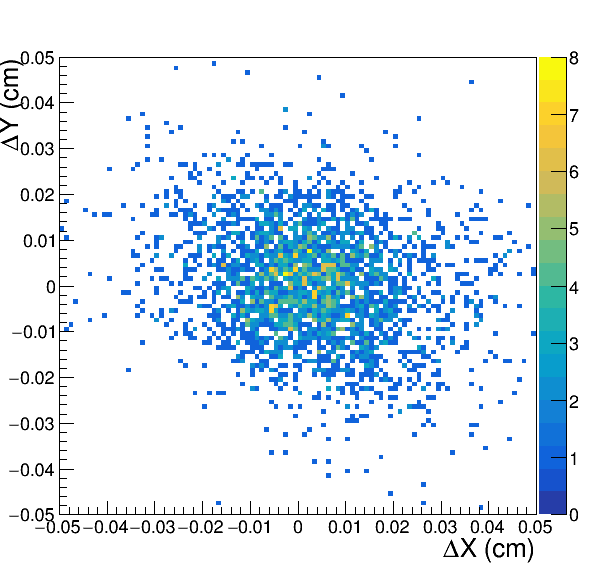
\includegraphics[width=\linewidth]{thesis_figures/alignment/Run_3211_after_millepede/square/GEM1.png}
  \caption{GEM1 after Millepede}
  %\label{fig:GEM1_after}
\end{subfigure}
%\hfill
\begin{subfigure}[r]{.45\textwidth}
  \centering
  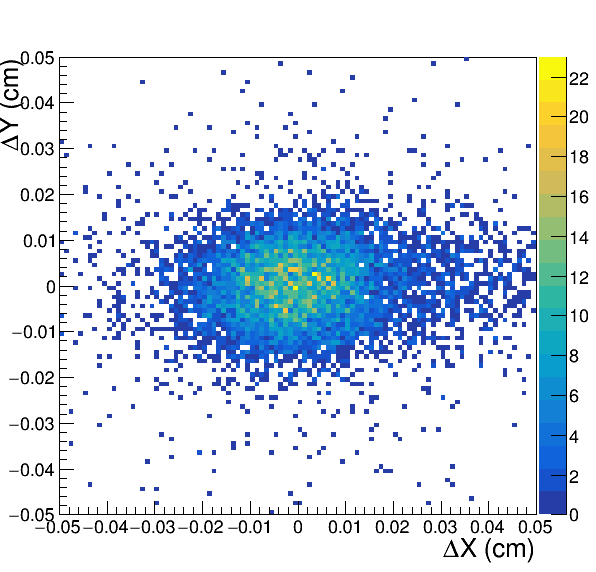
\includegraphics[width=\linewidth]{thesis_figures/alignment/Run_3211_after_millepede/Micromegas_off/GEM1.png}
  \caption{GEM1 after Millepede MM-off}
  \label{fig:GEM1_MXoff}
\end{subfigure}
\hfill
\begin{subfigure}[l]{.45\textwidth}
  \centering
  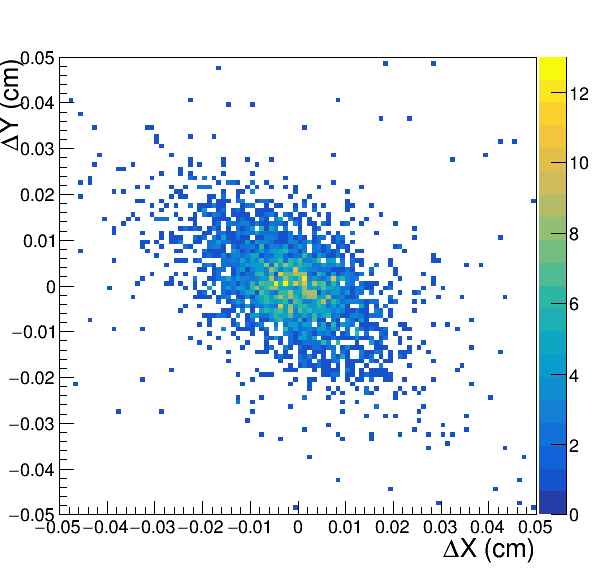
\includegraphics[width=\linewidth]{thesis_figures/alignment/Run_3211_after_millepede/square/GEM2.png}
  \caption{GEM2 after Millepede}
  %\label{fig:GEM2_after}
\end{subfigure}
%\hfill
\begin{subfigure}[r]{.45\textwidth}
  \centering
  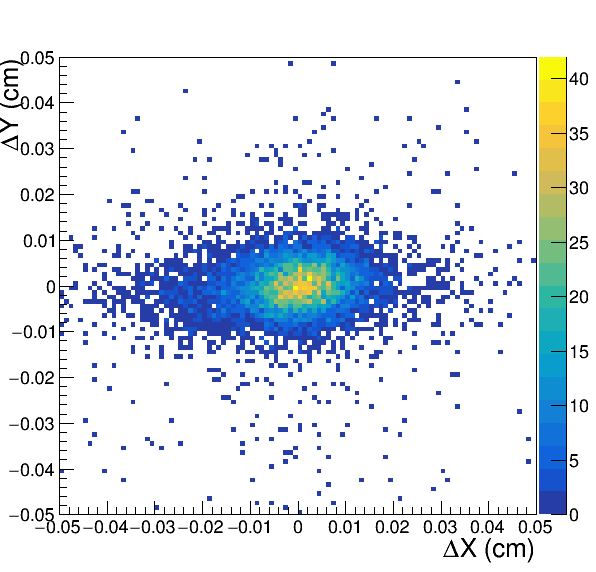
\includegraphics[width=\linewidth]{thesis_figures/alignment/Run_3211_after_millepede/Micromegas_off/GEM2.png}
  \caption{GEM2 after Millepede MM-off}
  \label{fig:GEM2_MXoff}
\end{subfigure}
\begin{subfigure}[l]{.45\textwidth}
  \centering
  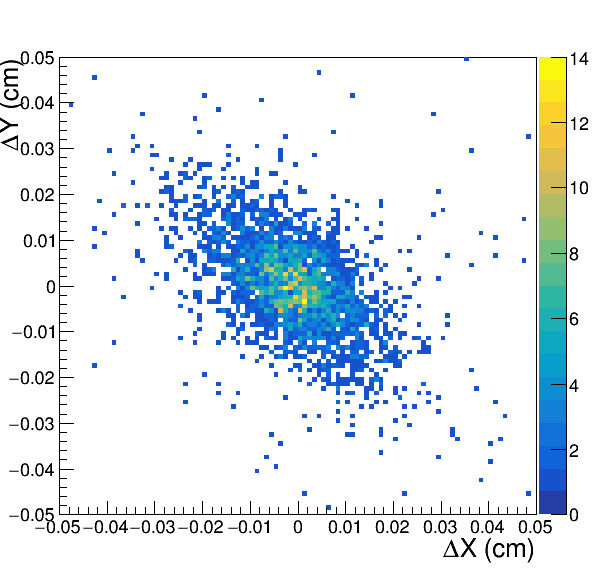
\includegraphics[width=\linewidth]{thesis_figures/alignment/Run_3211_after_millepede/square/GEM4.png}
  \caption{GEM4 after Millepede}
  %\label{fig:GEM4_after}
\end{subfigure}
%\hfill
\begin{subfigure}[r]{.45\textwidth}
  \centering
  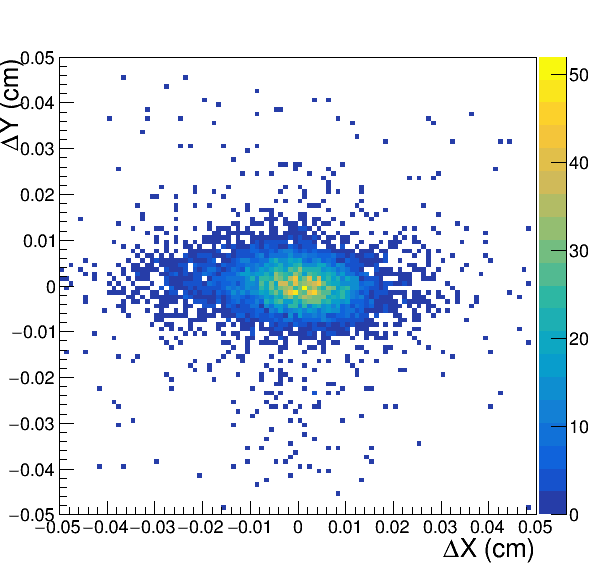
\includegraphics[width=\linewidth]{thesis_figures/alignment/Run_3211_after_millepede/Micromegas_off/GEM4.png}
  \caption{GEM4 after Millepede MM-off}
  \label{fig:GEM4_MXoff}
\end{subfigure}
\caption{Residual of GEM detectors with downstream Micromegas switched off}
\label{fig:MX_off}
\end{figure}
\FloatBarrier

\subsection[Angular Alignment]%
{Angular Alignment} %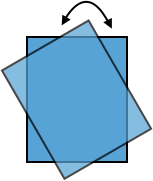
\includegraphics[width=20mm]{thesis_figures/Angular.png}}
Another global parameter that can impact the tracking resolution is the angular displacement. Each plane of the detector has a particular angle with respect to the global reference system. In the case of the GEM detectors used in our setup one plane is at $0^{\circ}$ with respect to the global system and this plane is named the X plane, on the other hand the Y plane, which is the readout plane perpendicular to X is at $90^{\circ}$ w.r.t the global system. This essentially means that the reference system for our GEMs is the same as that of the experiment. In the case of the Micromegas, the internal detector reference system is rotated by $45^{\circ}$ w.r.t the global system. To check whether an angular alignment was needed after the previously performed positional alignment for our setup, the obtained residuals were plotted against the position of hit for each plane of the detector. The results for the GEM detectors are shown in fig.(\ref{fig:res_vs_pos}) while the ones for the Micromegas are given in appendix(\ref{sec:app_1}). It was observed that for most of the detectors the residuals have no dependence on the position except for the case of GEM1, particularly for the X plane. To correct for this dependence an angular alignment was performed.

The angular(T) alignment was performed using the detectors table obtained after six iterations of the positional alignment(U) mentioned before. Initially during the T alignment only the X and Y planes of GEM1 were left free to rotate and all the other detector positions along with their respective angles were fixed. This was done to measure the impact of the alignment for one single detector. GEM1 was chosen since it was seen that the residuals for the X plane of the detector seemed to have a dependence on the position of the hits in the detector. The tracks used for alignment were chosen to have $\chi^2_{red} < 100$ and a $-110 \text{GeV} <\text{p/charge}< -90 \text{GeV}$. The result of the T alignment for GEM1, X plane is shown in fig.(\ref{fig:GEM1_T_align}). As it is seen in the figure the impact of the T alignment is minimal. However, it is important to mention that the result shown here was obtained after three iterations of the Millepede algorithm since the further iterations failed. The failure was during the CORAL part of the procedure which prohibits a change in the angle greater than $5^{\circ}$ for the GEM detectors. In spite of this restriction the three iterations should be more than enough to solve the angular displacement which is not the case. It was also found that the individual X and Y planes of the detector do not stay perpendicular to each other after the T alignment. This is unexpected since even though in CORAL they are treated as separate detectors, in reality the angle between them in the detector reference frame is fixed by construction. The observed angles for the planes were $89.563^{\circ}$ for the Y plane and $-0.324^{\circ}$ for the X plane after alignment i.e there is about a $0.2^{\circ}$ shift in the inherent angle between the two readout planes. This was confirmed to be a possibility which might have arisen during the detector construction particularly the chemical etching process~\cite{SAULI20162} used to construct the readout strips. This might also explain the angular dependence of the residuals observed in GEM1. Fig.(\ref{fig:red_chi2_3}) shows the $\chi^2_{red}$ before and after T alignment. We do see some shift towards a lower value but the overall shape of both the distributions is similar, reiterating the fact that the impact of the angular alignment is minimal for our setup at least in the case where we only align for one detector.

\begin{figure}[h!]
\centering
 \begin{subfigure}[l]{.45\textwidth}
   \centering
   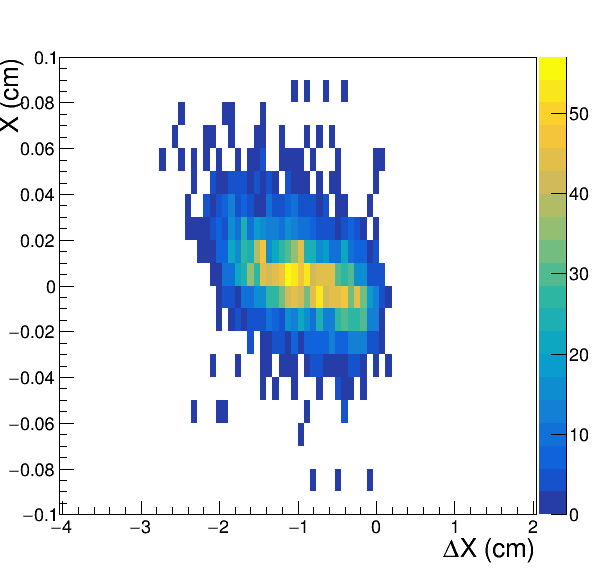
\includegraphics[width=\linewidth]{thesis_figures/alignment/Run_3211_T/G1X_after_millepede_U.png}

   \caption{GEM1 X plane}
   \label{fig:GEM1X_before}
 \end{subfigure}
 %\hfill
 \begin{subfigure}[r]{.45\textwidth}
   \centering
   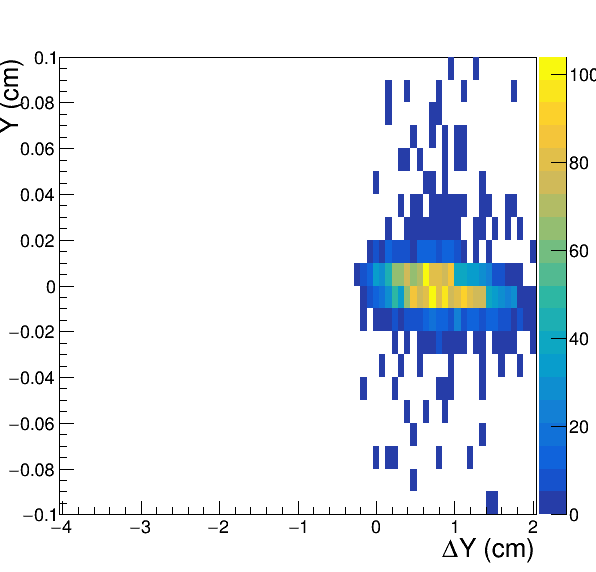
\includegraphics[width=\linewidth]{thesis_figures/alignment/Run_3211_T/G1Y_after_millepede_U.png}
   \caption{GEM1 Y plane}
   \label{fig:GEM1Y_before}
 \end{subfigure}
 \hfill
 \begin{subfigure}[l]{.45\textwidth}
   \centering
   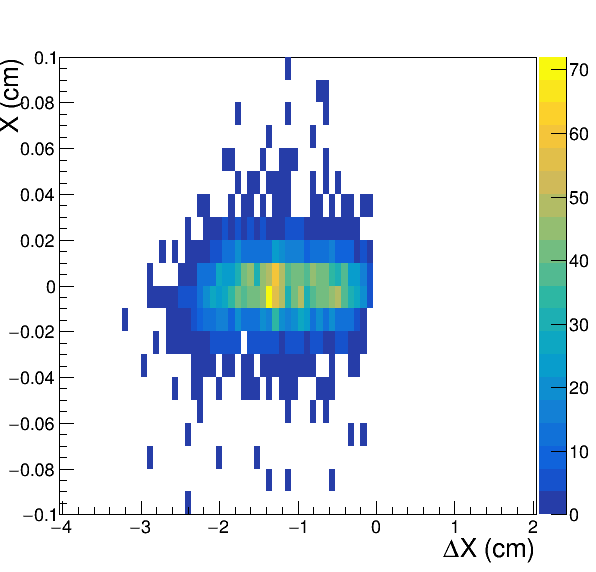
\includegraphics[width=\linewidth]{thesis_figures/alignment/Run_3211_T/G2X_after_millepede_U.png}
   \caption{GEM2 X plane}
   \label{fig:GEM2X_before}
 \end{subfigure}
 %\hfill
 \begin{subfigure}[r]{.45\textwidth}
   \centering
   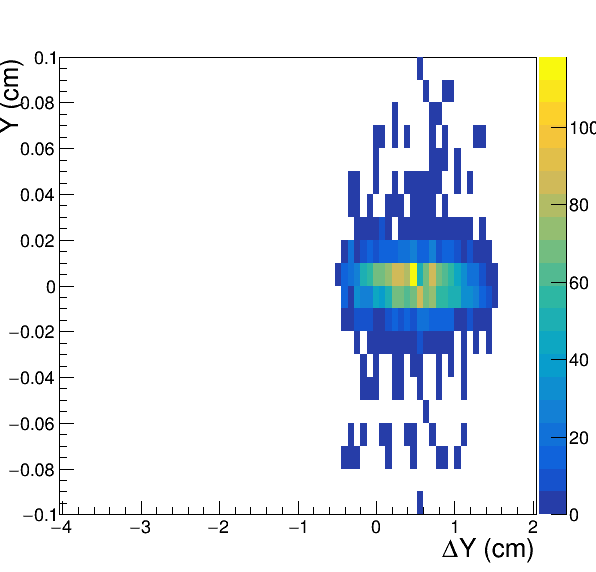
\includegraphics[width=\linewidth]{thesis_figures/alignment/Run_3211_T/G2Y_after_millepede_U.png}
   \caption{GEM2 Y plane}
   \label{fig:GEM2Y_before}
 \end{subfigure}
 \begin{subfigure}[l]{.45\textwidth}
   \centering
   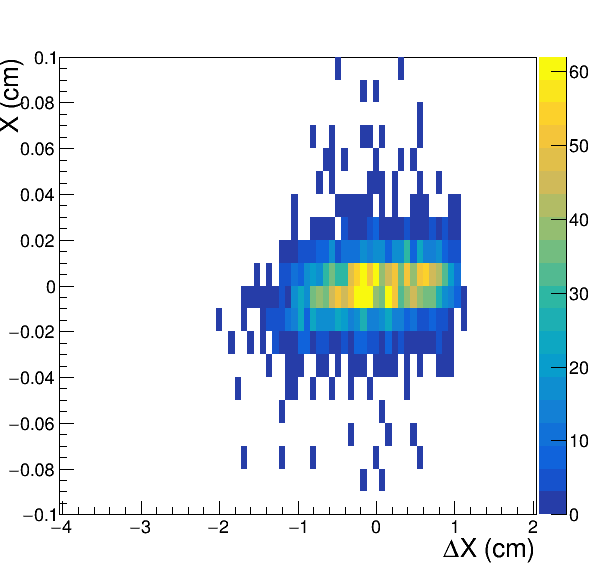
\includegraphics[width=\linewidth]{thesis_figures/alignment/Run_3211_T/G4X_after_millepede_U.png}

   \caption{GEM4 X plane}
   \label{fig:GEM4X_before}
 \end{subfigure}
 %\hfill
 \begin{subfigure}[r]{.45\textwidth}
   \centering
   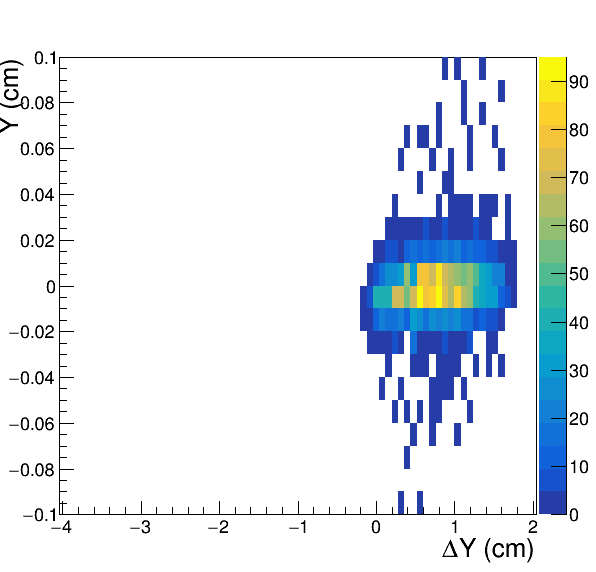
\includegraphics[width=\linewidth]{thesis_figures/alignment/Run_3211_T/G4Y_after_millepede_U.png}
   \caption{GEM4 Y plane}
   \label{fig:GEM4Y_before}
 \end{subfigure}
 \caption{Residual vs position for GEM detectors}
 \label{fig:res_vs_pos}
\end{figure}

%GEM1X plane alignment

\begin{figure}[h!]
\centering
 \begin{subfigure}[l]{.45\textwidth}
   \centering
   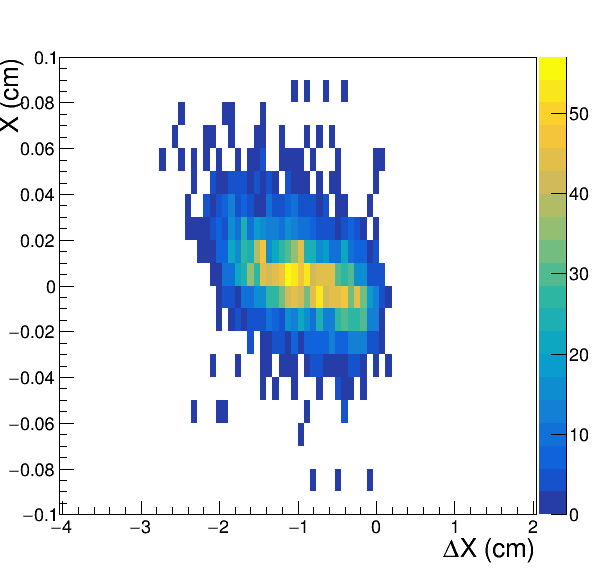
\includegraphics[width=\linewidth]{thesis_figures/alignment/Run_3211_T/G1X_after_millepede_U.png}

   \caption{GEM1 X plane before angular alignment}
   %\label{fig:GEM1X_before}
 \end{subfigure}
 %\hfill
 \begin{subfigure}[r]{.45\textwidth}
   \centering
   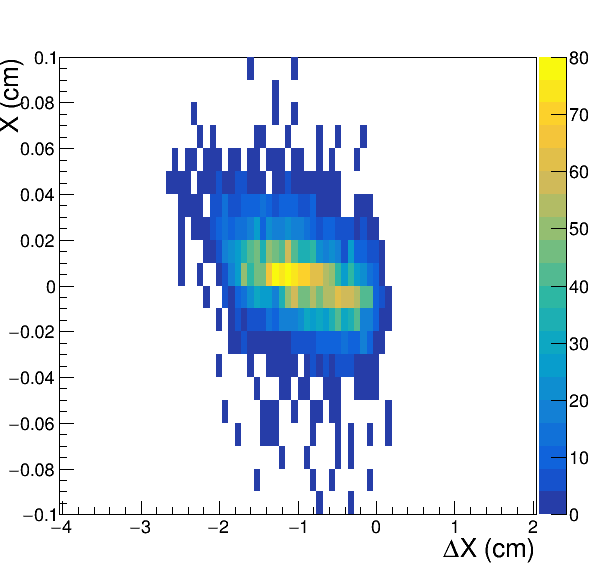
\includegraphics[width=\linewidth]{thesis_figures/alignment/Run_3211_T/G1X_after_millepede_T.png}
   \caption{GEM1 X plane after angular alignment}
   \label{fig:GEM1X_after_T}
 \end{subfigure}
 \caption{Angular alignment}
 \label{fig:GEM1_T_align}
 \end{figure}

 \begin{figure}[h!]
 \centering
 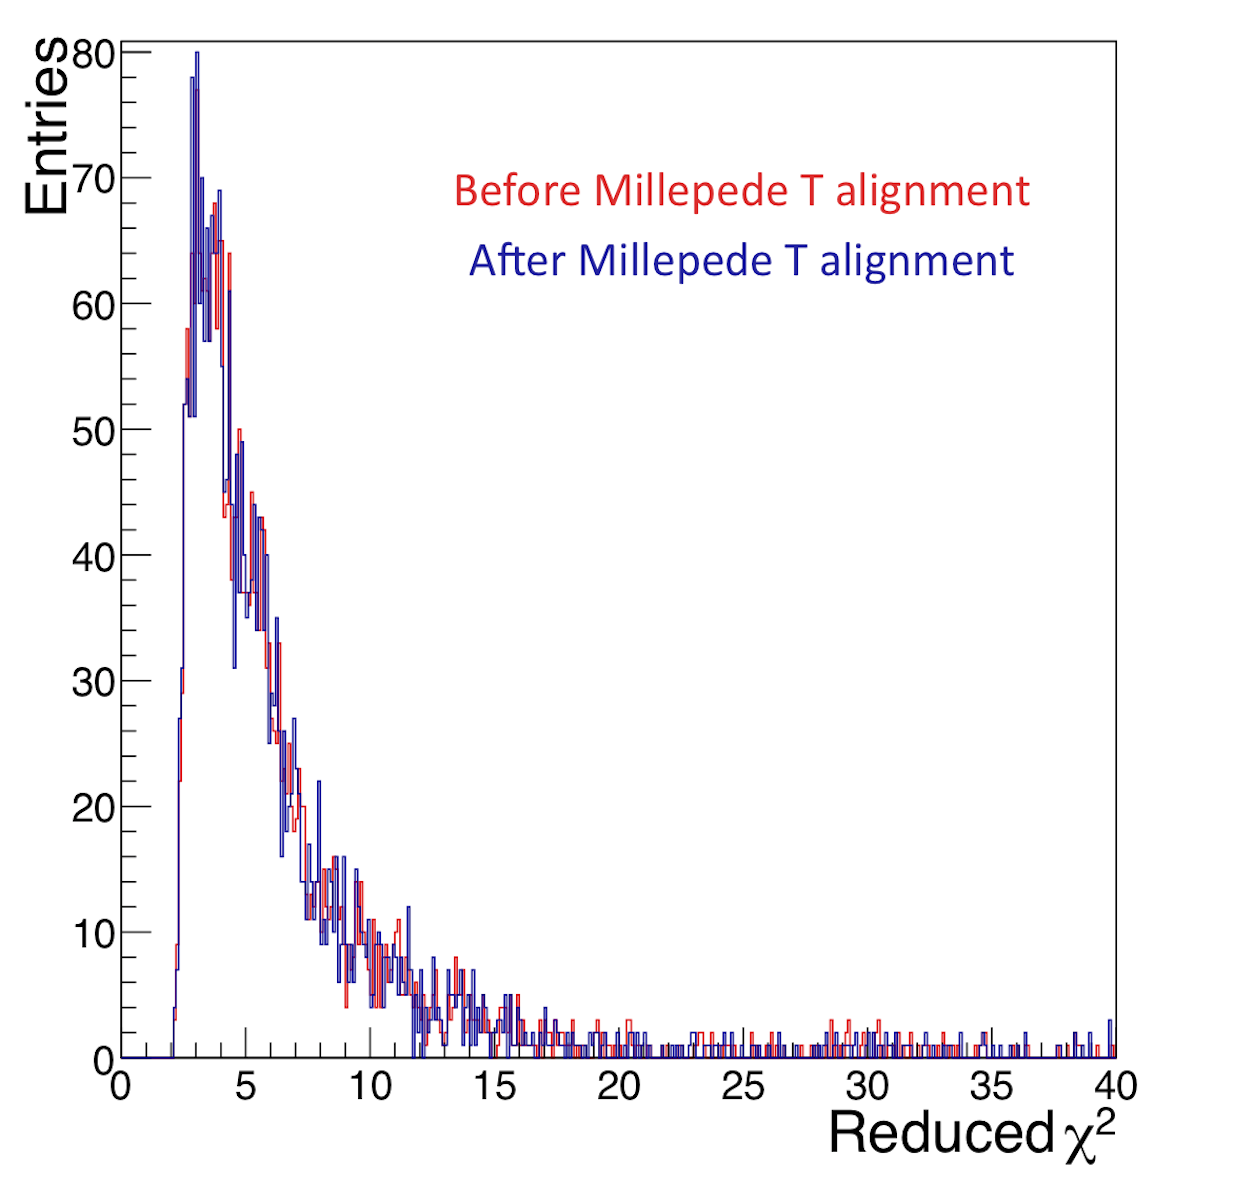
\includegraphics[width=0.8\textwidth]{thesis_figures/alignment/red_chi2_T.png}
 \caption{$\chi_{red}^2$ comparison before and after Millepede T alignment implementation}
 \label{fig:red_chi2_3}
 \end{figure}
\FloatBarrier

\subsection{Positional+Angular Alignment}
The end goal with the whole alignment procedure is to obtain the best possible alignment for each detector. Hence, the procedure was studied with both U and T alignment turned on.
Since the slight shift in the angle which was observed during U alignment was only present in a small number of detectors and is more prominent in GEM1 the impact of a U+T alignment was similar to that of U alignment. This alignment was performed just to check whether the alignment algorithm works if multiple global parameters are minimized in unison. The alignment was observed to be operational and the $\chi^2_{red}$ obtained was similar to that shown in fig.(\ref{fig:red_chi2_1}). The impact of the T alignment might not be visible for the particular run that was analyzed since the angular displacement for the detectors was minimal. However, for a future run by run alignment a full U+T alignment should be performed to correct for any possible angular displacement since for NA64 the experimental setup is constantly changing.

%%% Local Variables:
%%% mode: latex
%%% TeX-master: "mythesis"
%%% End:
